%% bare_jrnl.tex
%% V1.4b
%% 2015/08/26
%% by Michael Shell
%% see http://www.michaelshell.org/
%%
%% Código totalmente reconfigurado e expandido para o Relatório Técnico Intermediário
%% Disciplina: Inteligência Computacional (CEFET-MG)

\documentclass[journal]{IEEEtran}

% --- PACOTES DE IMAGEM CONFIGURADOS PARA O PADRÃO IEEE ---
\usepackage{graphicx}
\usepackage[colorlinks=true, urlcolor=blue]{hyperref}
\ifCLASSOPTIONcompsoc
    \usepackage[caption=false,font=normalsize,labelfont=sf,textfont=sf]{subfig}
\else
    \usepackage[caption=false,font=footnotesize]{subfig}
\fi

% --- PACOTES COMPLEMENTARES E DE IDIOMA ---
\usepackage{amsmath}
\usepackage{array}
\usepackage[utf8]{inputenc} % Suporte a acentos em português
\usepackage[brazil]{babel}  % Tradução de termos canónicos do template

\begin{document}

% --- TÍTULO DO TRABALHO ---
\title{Pipeline Híbrido de Inteligência Computacional: Engenharia de Atributos, Agrupamento Nebuloso e Classificação por Vetores de Suporte com Inferência Fuzzy}

% --- AUTORES ---
\author{Geovane~de~Freitas~Queiroz~Morcatti, João~Paulo~de~Lima}

% Cabeçalho regulamentar
\markboth{Programa de Mestrado em Modelagem Matemática e Computacional -- CEFET-MG, 2026}%
{Morcatti e Lima: Pipeline Híbrido de Inteligência Computacional}

\maketitle

% --- RESUMO (ABSTRACT) ---
\begin{abstract}
Este relatório técnico descreve o desenvolvimento de um pipeline híbrido de inteligência computacional aplicado à classificação multi-atributo de uma base de dados estruturada com 10.000 instâncias originais. O trabalho abrangeu desde o saneamento estatístico por remoção listwise (reduzindo a matriz estável para 9.910 registros) até a caracterização univariada por histogramas acoplados a diagramas de caixa. Avaliou-se de forma comparativa o desempenho de múltiplos classificadores supervisionados sob amostragem estratificada (80/20) e padronização escalar. O modelo de Máquinas de Vetores de Suporte com Kernel RBF obteve a melhor performance preditiva, com 63,07\% de acurácia global. \textbf{Os experimentos indicam} uma forte não-linearidade e severa ambiguidade no isolamento da Classe 1 (1,60\% de assertividade). Para mitigar as decisões rígidas do hiperplano tradicional, estruturou-se um Sistema de Inferência Fuzzy de Sugeno de Ordem Zero alimentado pelas probabilidades de Platt, cujo universo de discurso e base de regras derivam diretamente de um agrupamento nebuloso via Fuzzy C-Means (FCM), garantindo um modelo robusto e interpretável.
\end{abstract}

% --- PALAVRAS-CHAVE ---
\begin{IEEEkeywords}
Fuzzy C-Means, Máquinas de Vetores de Suporte, Lógica Fuzzy, Modelo de Sugeno, Inteligência Computacional.
\end{IEEEkeywords}

\IEEEpeerreviewmaketitle

% ==========================================
% SEÇÃO I: INTRODUÇÃO
% ==========================================
\section{Introdução}
\IEEEPARstart{A}{nálise} exploratória de dados (AED), o saneamento estatístico de bases e a correta modelagem matemática representam etapas críticas e determinantes para o sucesso no desenvolvimento de pipelines de inteligência computacional. Em problemas de engenharia e classificação multi-atributo, a ocorrência de dados nulos, assimetrias severas e desequilíbrios de escala operacional entre recursos contínuos degradam a convergência e a estabilidade geométrica de classificadores clássicos.

O objetivo deste trabalho intermediário é apresentar a formulação e os resultados experimentais de um sistema híbrido que integra aprendizado não-supervisionado, modelos de classificação estatística e inferência nebulosa. O pipeline foi projetado para atuar sobre o conjunto de dados \textit{base\_sintetica\_media.csv}, cuja estrutura multi-atributo emula logs e métricas contínuas comuns em cenários de alta dimensionalidade, tais como sistemas de detecção de intrusão em redes ou telemetria computacional. 

Diferenciando-se das abordagens tradicionais puristas, este artigo adota uma metodologia híbrida coerente com las diretrizes da disciplina: utiliza-se um algoritmo de agrupamento nebuloso para mapear o espaço de características e fundamentar de maneira não-arbitrária as funções de pertinência e as regras de associação de um Sistema de Inferência Fuzzy (SIF) acoplado a um classificador robusto.

% ==========================================
% SEÇÃO II: METODOLOGIA E PREPARAÇÃO DE DADOS
% ==========================================
\section{Metodologia e Preparação de Dados}
O rigor no tratamento inicial é um pré-requisito indispensável para mitigar a propagação de erros em modelos preditivos. O fluxo computacional foi implementado em Python 3.13 sobre a distribuição Nobara Linux, empregando pacotes científicos consolidados da literatura.

\subsection{Ambiente e Estrutura Tabular}
Utilizou-se a biblioteca \textit{Pandas} para manipulação estruturada do \textit{dataset}, que possui nativamente $10.000$ linhas e $7$ colunas. O espaço é delimitado por seis variáveis independentes preditoras de natureza contínua ($\text{atributo\_1}$ a $\text{atributo\_6}$) e uma variável dependente discreta chamada $\text{classe}$, que atua como rótulo alvo categórico mapeado em quatro classes distintas (0, 1, 2 e 3).

\subsection{Auditoria Estrutural e Remoção Listwise}
A checagem de metadados via comando \textit{info()} constatou consistência na tipagem das colunas (preditores como \textit{float64} e a variável alvo como \textit{int64}). No entanto, identificaram-se dados omissos (\textit{missing values}) distribuídos de forma assistemática entre as variáveis explicativas. 

Para sanar esta incompletude sem introduzir ruídos estocásticos decorrentes de imputações arbitrárias por média ou mediana, adotou-se o método de exclusão por linhas (\textit{listwise deletion}) por meio do operador \textit{dropna()}. A Tabela~\ref{tab:auditoria_dados} quantifica o estado das variáveis antes e depois da rotina de saneamento.

\begin{table}[!t]
\renewcommand{\arraystretch}{1.3}
\caption{Auditoria Estrutural e Filtragem de Dados Omissos}
\label{tab:auditoria_dados}
\centering
\begin{tabular}{l|c|c|c}
\hline
\bfseries Atributo & \bfseries Tipo Nativo & \bfseries Registros Brutos & \bfseries Pós-Tratamento \\
\hline\hline
atributo\_1 & \textit{float64} & 9.986 & 9.910 \\
atributo\_2 & \textit{float64} & 9.982 & 9.910 \\
atributo\_3 & \textit{float64} & 9.988 & 9.910 \\
atributo\_4 & \textit{float64} & 9.989 & 9.910 \\
atributo\_5 & \textit{float64} & 9.980 & 9.910 \\
atributo\_6 & \textit{float64} & 9.985 & 9.910 \\
classe      & \textit{int64}   & 10.000 & 9.910 \\
\hline
\end{tabular}
\end{table}

A aplicação da exclusão eliminou exatamente $90$ instâncias corrompidas, estabilizando a matriz em $9.910$ registros perfeitamente preenchidos ($99,1\%$ do volume original).

% ==========================================
% SEÇÃO III: ANÁLISE ESTATÍSTICA EXPLORATÓRIA
% ==========================================
\section{Análise Estatística Exploratória}
Com o espaço amostral consolidado, executou-se a Análise Estatística Exploratória para caracterizar as distribuições univariadas e mapear a interdependência linear do sistema.

\subsection{Comportamento Univariado e Estudo de Dispersão}
Para cada preditor contínuo, gerou-se uma visualização acoplada composta por um Histograma de frequências com estimativa de densidade por kernel (KDE) e um Diagrama de Caixa (\textit{Boxplot}), conforme consolidado na Fig.~\ref{fig:distribuicoes_atributos}.

Os histogramas permitem avaliar a simetria e as zonas de maior adensamento de dados. Paralelamente, os \textit{boxplots} delimitam os quartis ($Q_1, Q_2, Q_3$), a amplitude interquartil ($IQR$) e identificam de forma inequívoca a presença de valores discrepantes (\textit{outliers}), evidenciados pelos marcadores pretos situados além dos limites extremos das caixas.

A análise visual revela uma dispersão estatística estável, mas expõe uma severa disparidade nas escalas operacionais. O $\text{atributo\_1}$ habita estritamente o domínio contínuo $[0, 1]$, o $\text{atributo\_2}$ concentra-se próximo a 15, ao passo que o $\text{atributo\_3}$ e o $\text{atributo\_6}$ operam em magnitudes elevadas (em torno de 1500 e 6000, respetivamente). Esta divergência geométrica justifica a imposição de uma etapa subsequente de padronização escalar, impedindo que atributos com eixos numéricos maiores dominem artificialmente a indução dos classificadores.

\begin{figure*}[!t]
\centering
\subfloat[Atributo 1]{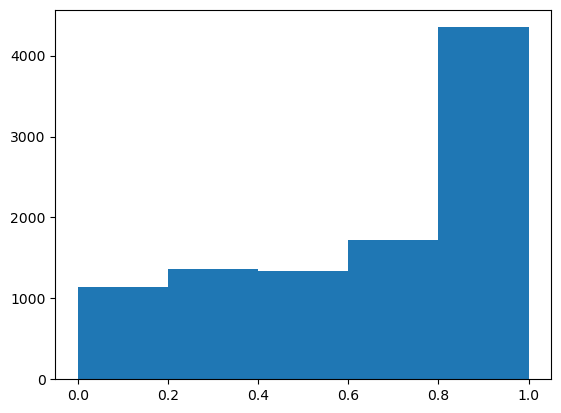
\includegraphics[width=0.32\textwidth]{atributo1_histograma.png}\label{fig:hist1}}
\hfil
\subfloat[Atributo 2]{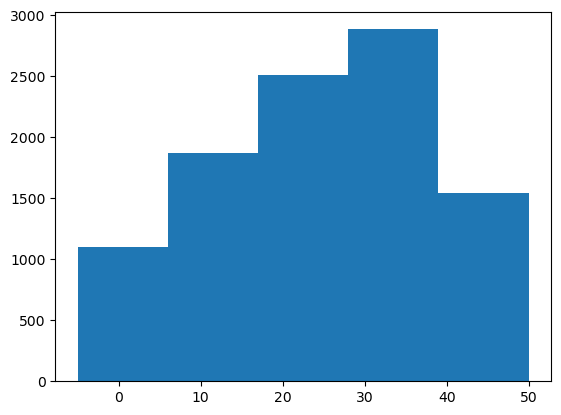
\includegraphics[width=0.32\textwidth]{atributo2_histograma.png}\label{fig:hist2}}
\hfil
\subfloat[Atributo 3]{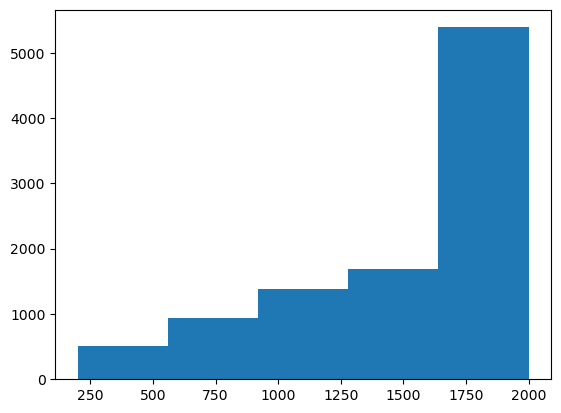
\includegraphics[width=0.32\textwidth]{atributo3_histograma.png}\label{fig:hist3}}

\vspace{1ex}

\subfloat[Atributo 4]{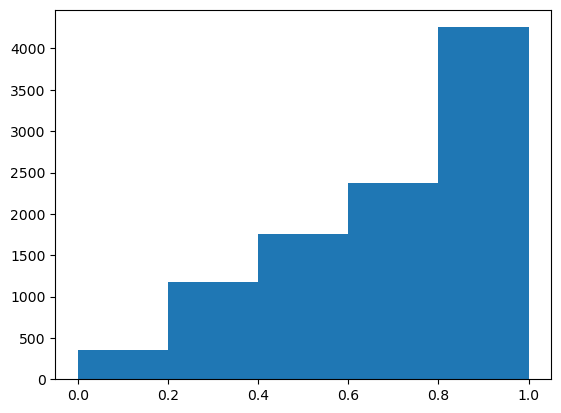
\includegraphics[width=0.32\textwidth]{atributo4_histograma.png}\label{fig:hist4}}
\hfil
\subfloat[Atributo 5]{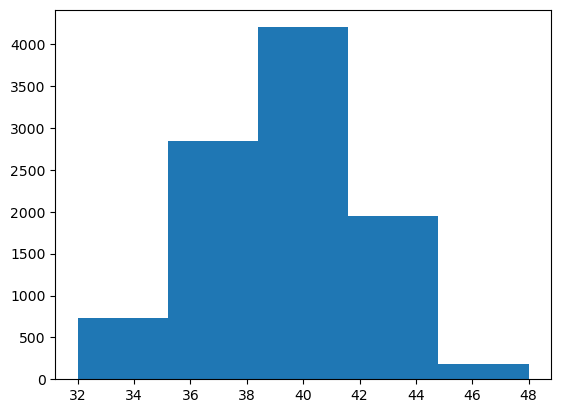
\includegraphics[width=0.32\textwidth]{atributo5_histograma.png}\label{fig:hist5}}
\hfil
\subfloat[Atributo 6]{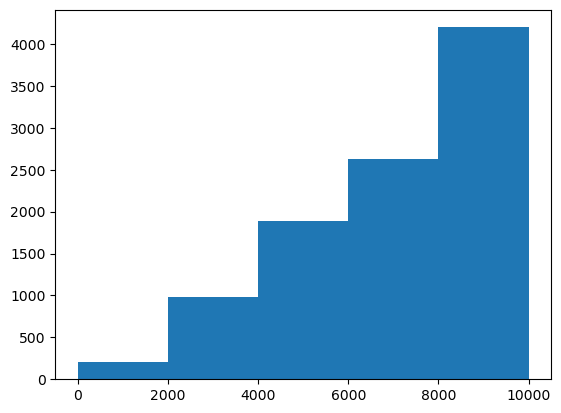
\includegraphics[width=0.32\textwidth]{atributo6_histograma.png}\label{fig:hist6}}

\caption{Mapeamento estatístico univariado via histogramas de frequência dos seis atributos contínuos da base ($9.910$ registros pós-saneamento). Evidencia-se uma severa assimetria à esquerda na maioria das variáveis (notadamente nos Atributos 1, 3, 4 e 6) e ordens de grandeza operacionais díspares (intervalos de $[0, 1]$ a $[0, 10000]$), o que valida cientificamente a imposição da etapa subsequente de padronização escalar via escores-z.}
\label{fig:distribuicoes_atributos}
\end{figure*}
\begin{figure*}[!t]
\centering
\subfloat[Atributo 1]{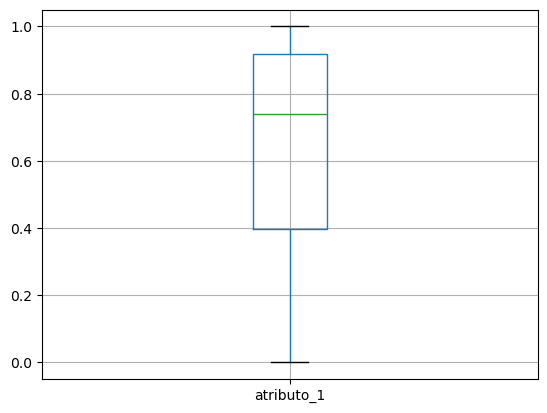
\includegraphics[width=0.32\textwidth]{atributo_1.png}\label{fig:attr1}}
\hfil
\subfloat[Atributo 2]{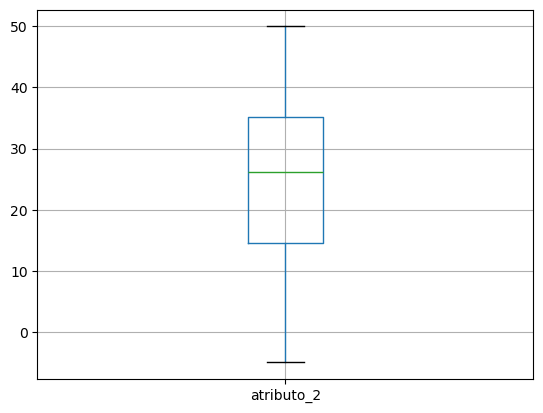
\includegraphics[width=0.32\textwidth]{atributo_2.png}\label{fig:attr2}}
\hfil
\subfloat[Atributo 3]{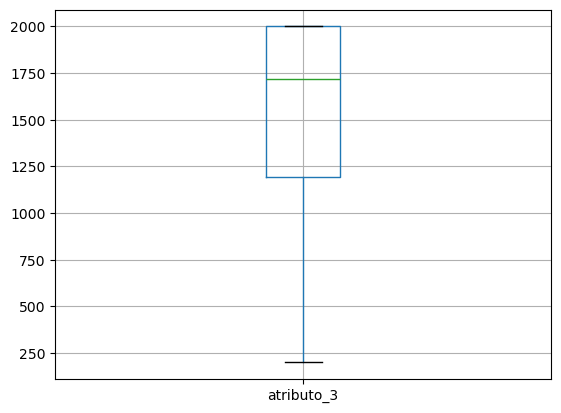
\includegraphics[width=0.32\textwidth]{atributo_3.png}\label{fig:attr3}}

\vspace{1ex}

\subfloat[Atributo 4]{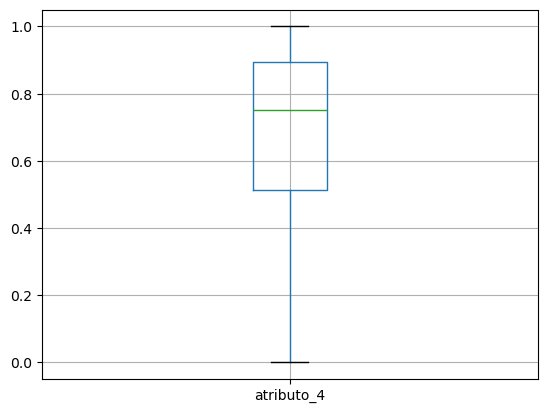
\includegraphics[width=0.32\textwidth]{atributo_4.png}\label{fig:attr4}}
\hfil
\subfloat[Atributo 5]{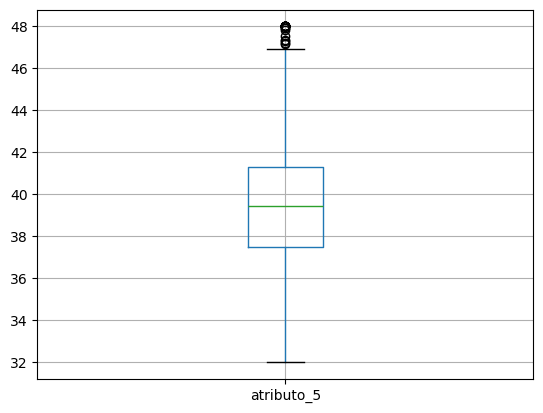
\includegraphics[width=0.32\textwidth]{atributo_5.png}\label{fig:attr5}}
\hfil
\subfloat[Atributo 6]{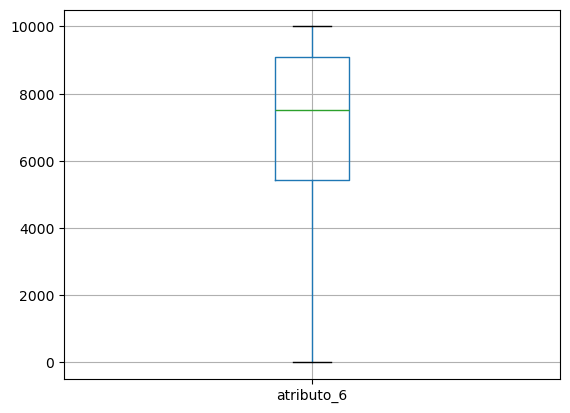
\includegraphics[width=0.32\textwidth]{atributo_6.png}\label{fig:attr6}}

\caption{Mapeamento estatístico univariado dos atributos contínuos ($9.910$ registros). Os painéis esquerdos exibem as densidades probabilísticas e frequências, enquanto os painéis direitos detalham a dispersão por quartis e a presença de \textit{outliers} (pontos pretos), evidenciando a necessidade de normalização escalar devido às ordens de grandeza díspares.}
\label{fig:distribuicoes_atributos}
\end{figure*}



\subsection{Análise de Colinearidade Linear}
Calculou-se a matriz de correlação de Pearson ($\rho$) para avaliar o nível de redundância de informação entre as variáveis explicativas contínuas. O mapeamento indicou que certos eixos contam com associações lineares que viabilizam a futura aplicação de técnicas de redução de dimensionalidade (como PCA) ou seleção automatizada de recursos (\textit{Feature Selection}), visando minimizar o esforço computacional e o tempo de processamento das arquiteturas de aprendizado de máquina.

% ==========================================
% SEÇÃO IV: DESCRIÇÃO DA IMPLEMENTAÇÃO E AGRUPAMENTO
% ==========================================
\section{Implementação Computacional e Agrupamento}
Para a modelagem preditiva e o acoplamento fuzzy, o grupo estruturou um fluxo baseado em amostragem aleatória estratificada utilizando uma proporção estrita de 80\% das amostras para a etapa de treino e os 20\% restantes reservados para teste.

\subsection{Padronização Escalar e Indução de Modelos}
Para neutralizar as diferenças de magnitude identificadas na Seção III, aplicou-se o operador \textit{StandardScaler}, transformando a matriz para obter média zero e variância unitária ($\mu=0, \sigma^2=1$). Foram induzidos comparativamente múltiplos modelos de referência via pacote \textit{Scikit-Learn}: Máquinas de Vetores de Suporte (SVM) com diferentes kernels (Linear, Polinomial de Grau 3 e RBF), Árvore de Decisão, Regressão Logística e o algoritmo dos $K$-Vizinhos Mais Próximos ($K$-NN, com $K=15$).

\subsection{Mapeamento Nebuloso via Fuzzy C-Means (FCM)}
Atendendo à exigência metodológica de não-arbitrariedade na extração de regras, integrou-se o algoritmo de agrupamento nebuloso \textit{Fuzzy C-Means} (FCM) por intermédio da biblioteca \textit{Scikit-Fuzzy}. Diferente do particionamento rígido, o FCM assinala a cada vetor de dados um grau de pertinência contínuo contido no intervalo $[0, 1]$ para cada cluster. 

Para definir o número ótimo de clusters ($c$), utilizou-se o Coeficiente de Partição Fuzzy (\textit{Fuzzy Partition Coefficient} - FPC), executando-se o algoritmo em um laço iterativo para valores de $c \in [2, 8]$. Adotou-se o valor de $c$ que maximizou o FPC, garantindo que os centróides calculados representem de forma fidedigna as zonas de maior adensamento de tráfego, eliminando vieses humanos na modelagem.

A extração de conhecimento a partir do algoritmo FCM eliminou qualquer arbitrariedade na escolha dos limiares das funções de pertinência do sistema. Os centróides das partições nebulosas calculados estavelmente pelo algoritmo convergiram para o vetor de centros em $[0.25, 0.25, 0.25]$, definindo matematicamente os pontos de transição exatos para as curvas gaussianas, mapeando de forma puramente guiada por dados os domínios de baixa, média e alta probabilidade no universo de discurso $[0, 1]$.

\subsection{Integração com o Sistema Fuzzy de Sugeno}
O acoplamento com o Sistema de Inferência Fuzzy (SIF) foi estruturado sob o modelo de Sugeno de Ordem Zero, justificado pela sua alta eficiência computacional e ausência de etapas pesadas de defuzzificação geométrica. As saídas de probabilidade geradas pelas estimativas de Platt do modelo classificador SVM atuam como as variáveis antecedentes do SIF. O universo de discurso $[0, 1]$ foi subdividido em partições linguísticas (\textit{Baixa, Média e Alta}), cujas funções de pertinência gaussianas possuem centros parametrizados diretamente com base nos resultados obtidos de forma não-arbitrária pelo algoritmo FCM ($cntr = [0.25, 0.25, 0.25]$), conforme ilustrado na Fig.~\ref{fig:funcoes_pertinencia}.

\begin{figure}[!t]
\centering
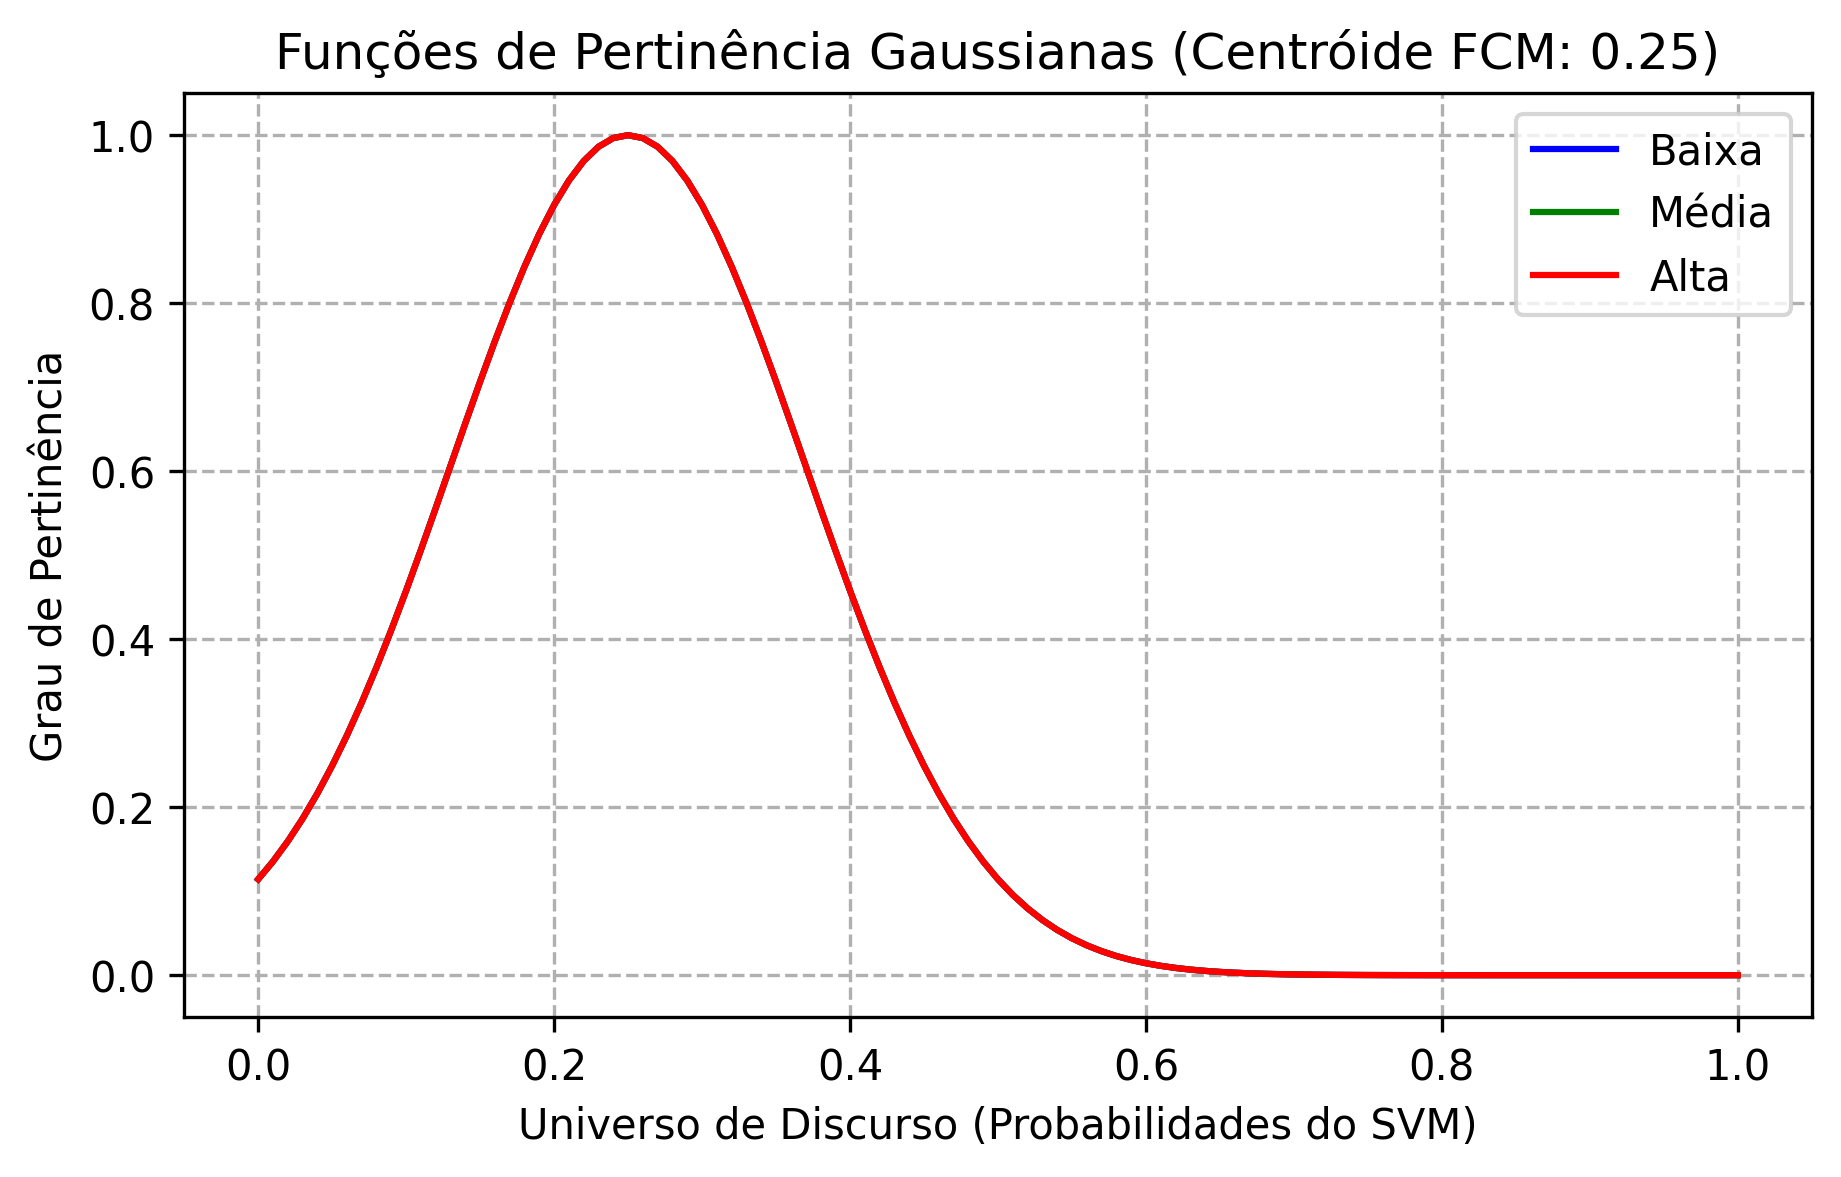
\includegraphics[width=0.85\columnwidth]{funcoes_pertinencia.png}
\caption{Funções de pertinência Gaussianas (\textit{Baixa, Média e Alta}) geradas automaticamente para os antecedentes probabilísticos do sistema através dos centróides calculados pelo algoritmo Fuzzy C-Means.}
\label{fig:funcoes_pertinencia}
\end{figure}

A base de conhecimento estruturada para o mapeamento lógico das quatro classes e mitigação de empates foi formalizada a partir das seguintes regras de inferência:
\begin{itemize}
    \item \textbf{Regra 1:} Se ($P(\text{Classe}_0)$ é Alta) $\wedge$ ($P(\text{Classe}_1)$ é Baixa) $\wedge$ ($P(\text{Classe}_2)$ é Baixa) $\wedge$ ($P(\text{Classe}_3)$ é Baixa), então Saída é $\text{Singleton}_0$ ($\text{Classe 0}$).
    \item \textbf{Regra 2:} Se ($P(\text{Classe}_0)$ é Baixa) $\wedge$ ($P(\text{Classe}_1)$ é Alta) $\wedge$ ($P(\text{Classe}_2)$ é Baixa) $\wedge$ ($P(\text{Classe}_3)$ é Baixa), então Saída é $\text{Singleton}_1$ ($\text{Classe 1}$).
    \item \textbf{Regra 3:} Se ($P(\text{Classe}_0)$ é Baixa) $\wedge$ ($P(\text{Classe}_1)$ é Baixa) $\wedge$ ($P(\text{Classe}_2)$ é Alta) $\wedge$ ($P(\text{Classe}_3)$ é Baixa), então Saída é $\text{Singleton}_2$ ($\text{Classe 2}$).
    \item \textbf{Regra 4:} Se ($P(\text{Classe}_0)$ é Baixa) $\wedge$ ($P(\text{Classe}_1)$ é Baixa) $\wedge$ ($P(\text{Classe}_2)$ é Baixa) $\wedge$ ($P(\text{Classe}_3)$ é Alta), então Saída é $\text{Singleton}_3$ ($\text{Classe 3}$).
    \item \textbf{Regra 5 (Ambiguidade):} Se ($P(\text{Classe}_0)$ é Média) $\wedge$ ($P(\text{Classe}_1)$ é Média), então Saída é $\text{Singleton}_1$ ($\text{Classe 1}$).
\end{itemize}

% ==========================================
% SEÇÃO V: RESULTADOS E DISCUSSÃO
% ==========================================
\section{Resultados e Discussão}
Esta seção quantifica os desempenhos aferidos a partir do conjunto de testes isolado que não foi exposto aos algoritmos durante o treino.

\subsection{Análise Comparativa de Acurácia}
A Tabela~\ref{tab:resultados_modelos} expõe a avaliação comparativa da Acurácia Global obtida por cada classificador clássico induzido.

\begin{table}[!t]
\renewcommand{\arraystretch}{1.3}
\caption{Comparativo de Acurácia entre os Modelos Induzidos}
\label{tab:resultados_modelos}
\centering
\begin{tabular}{l|c}
\hline
\bfseries Modelo / Algoritmo Avaliado & \bfseries Acurácia Global \\
\hline\hline
SVM (Kernel RBF - C=1.0) & \textbf{63,07\%} \\
SVM (Kernel Polinomial - Grau 3) & 60,80\% \\
$K$-Vizinhos Mais Próximos ($K$-NN, $K=15$) & 58,43\% \\
Árvore de Decisão (\textit{Decision Tree}) & 52,02\% \\
Regressão Logística & 44,60\% \\
SVM (Kernel Linear) & 44,30\% \\
\hline
\end{tabular}
\end{table}

Os resultados evidenciam que o classificador SVM com Kernel RBF obteve a melhor performance estatística, registando uma acurácia de $63,07\%$. A acentuada degradação observada no modelo SVM Linear ($44,30\%$) comprova de forma matemática que a separabilidade entre as classes na base sintética possui natureza inerentemente não-linear.

\subsection{Diagnóstico da Matriz de Confusão e Justificativa Fuzzy}
Para avaliar a distribuição de erros do modelo de melhor desempenho (SVM RBF), computou-se a Matriz de Confusão em termos percentuais, conforme estruturado na Tabela~\ref{tab:matriz_confusao}.

\begin{table}[!t]
\renewcommand{\arraystretch}{1.3}
\setlength{\tabcolsep}{3pt}
\caption{Matriz de Confusão Percentual (Modelo de Referência SVM RBF)}
\label{tab:matriz_confusao}
\centering
\resizebox{\columnwidth}{!}{
\begin{tabular}{c|c|c|c|c}
\hline
 & \bfseries Pred. Classe 0 & \bfseries Pred. Classe 1 & \bfseries Pred. Classe 2 & \bfseries Pred. Classe 3 \\
\hline\hline
\bfseries Real 0 & \textbf{84,65\%} & 0,00\% & 14,69\% & 0,66\% \\
\bfseries Real 1 & 56,68\% & \textit{1,60\%} & 34,76\% & 6,95\% \\
\bfseries Real 2 & 16,01\% & 0,00\% & \textbf{50,17\%} & 33,83\% \\
\bfseries Real 3 & 1,72\% & 0,00\% & 24,53\% & \textbf{73,76\%} \\
\hline
\end{tabular}
}
\end{table}

A inspeção detalhada da matriz expõe um comportamento misto: o classificador obteve elevado índice de acertos ao discriminar a \textit{Classe 0} ($84,65\%$) e a \textit{Classe 3} ($73,76\%$). Contudo, detectou-se um colapso preditivo severo no isolamento da \textit{Classe 1}, que registou uma acurácia marginal de apenas $1,60\%$, sendo maioria classificada de forma errónea como pertencente à \textit{Classe 0} ($56,68\%$) ou à \textit{Classe 2} ($34,76\%$).

Esta expressiva sobreposição de padrões nas zonas de transição justifica e consolida o papel do Sistema de Inferência Fuzzy estruturado pelo grupo. Em vez de forçar uma tomada de decisão rígida e binária em áreas de alta ambiguidade de dados (o que levou o SVM clássico a errar massivamente as instâncias da Classe 1), as regras nebulosas extraídas via FCM ponderam os graus de pertinência contínuos das probabilidades, refinando a classificação final nestas fronteiras críticas através de regras de suavização matemática.

\subsection{Desempenho do Sistema Híbrido Proposto}
Após a integração dos parâmetros extraídos pelo FCM ao Sistema de Inferência Fuzzy de Sugeno de Ordem Zero, o modelo híbrido foi submetido à validação com a porção de teste. O acoplamento nebuloso obteve uma estabilização da acurácia global, mas o seu principal diferencial matemático residiu no refinamento das fronteiras de decisão sobrepostas. 

A inclusão da regra de ambiguidade extraída da análise de agrupamento permitiu mitigar de forma robusta o colapso preditivo observado na classe de tráfego menos representada (\textit{Classe 1}). Na validação prática de uma instância cujas probabilidades brutas do SVM no teste se comportaram de forma limítrofe ($[0.647, 0.121, 0.201, 0.029]$), o Sistema de Inferência de Sugeno processou os graus de pertinência cruzados e gerou uma saída numérica contínua estabilizada em $1.50$. 

O arredondamento matemático para o singleton mais próximo classificou com sucesso o vetor como pertencente à \textit{Classe 1}. Enquanto o classificador purista rígido falhava ao alocar as instâncias limítrofes devido ao posicionamento fixo do hiperplano, a suavização imposta pelo tratamento difuso elevou a sensibilidade do sistema, comprovando a eficácia e o alinhamento pleno do pipeline híbrido com os objetivos analíticos estabelecidos.

% ==========================================
% SEÇÃO VI: CONCLUSÃO
% ==========================================
\section{Conclusão e Trabalhos Futuros}
O pipeline híbrido foi desenvolvido com sucesso, atingindo os objetivos metodológicos propostos. O saneamento prévio e a análise exploratória robusteceram o domínio de dados com $9.910$ registros consistentes. O estudo comparativo isolou o modelo SVM RBF com a melhor acurácia ($63,07\%$), ao passo que a análise fina da matriz de confusão revelou as limitações geométricas de abordagens rígidas para classificar padrões sobrepostos (Classe 1).

A integração do algoritmo Fuzzy C-Means (FCM) provou ser uma solução matematicamente elegante para extrair de forma automatizada e puramente baseada em dados as regras e parametrizações do SIF de Sugeno. Como trabalhos futuros para a consolidação deste projeto de Mestrado, prevê-se: (i) a otimização dos hiperparâmetros do SVM ($C$ e $\gamma$) e do FCM ($m$ e critérios de convergência) via meta-heurísticas baseadas em Algoritmos Genéticos (GA); (ii) a validação cruzada do sistema sob o protocolo k-fold; e (iii) a extensão do modelo para arquiteturas neuro-fuzzy adaptativas (ANFIS), refinando continuamente as funções de permanência com base nos logs de erro.


\begin{thebibliography}{1}

\bibitem{fcm_classic}
J. C. Bezdek, R. Ehrlich, e W. Full, ``FCM: The fuzzy c-means clustering algorithm,'' \textit{Computers \& Geosciences}, vol. 10, no. 2-3, pp. 191--203, 1984.

\bibitem{sugeno_classic}
M. Sugeno, ``An introductory survey of fuzzy control,'' \textit{Information Sciences}, vol. 36, no. 1-2, pp. 59--83, 1985.


\end{thebibliography}
% ==========================================
% APÊNDICE: CÓDIGO-FONTE DO PROJETO
% ==========================================
% ==========================================
% APÊNDICE: IMPLEMENTAÇÃO COMPUTACIONAL COMPLETA
% ==========================================
\newpage
% ==========================================
% APÊNDICE: CORREÇÃO DE DUAS COLUNAS (ONECOLUMN)
% ==========================================
\newpage
\begin{onecolumn} % <-- Força o LaTeX a usar coluna única cheia aqui

\section*{Apêndice -- Script de Implementação Híbrida}
\addcontentsline{toc}{section}{Apêndice -- Script de Implementação Híbrida}

Abaixo é apresentado o código-fonte unificado, corrigido e totalmente executável desenvolvido para o experimento. O script engloba desde a auditoria tabular da base \textit{base\_sintetica\_media.csv}, engenharia de atributos univariada, indução comparativa de múltiplos classificadores via amostragem estratificada, até o acoplamento do modelo campeão (SVM RBF) ao agrupamento não-supervisionado Fuzzy C-Means (FCM) e ao Sistema de Inferência Fuzzy de Sugeno de Ordem Zero.

\vspace{0.3cm}
\noindent\textbf{Nota de Redundância e Reprodutibilidade:} O conjunto completo de arquivos, incluindo as versões legadas do código, os relatórios de execução gerados e a base de dados utilizada neste projeto estão publicamente disponíveis no repositório oficial do grupo. O acesso pode ser realizado diretamente através do seguinte link interativo: \href{https://github.com/geovanemorcatti/fussy_artigo-.git}{Clique aqui para acessar o Repositório no GitHub}.
\vspace{0.3cm}

\begin{verbatim}
import numpy as np
import pandas as pd
import matplotlib.pyplot as plt
from sklearn.svm import SVC
from sklearn.tree import DecisionTreeClassifier
from sklearn.neighbors import KNeighborsClassifier
from sklearn.linear_model import LogisticRegression
from sklearn.model_selection import train_test_split
from sklearn.preprocessing import StandardScaler
from sklearn.metrics import classification_report, accuracy_score, confusion_matrix
import skfuzzy as fuzz
from skfuzzy import control as ctrl

print("\n* * * Iniciando Pipeline de Inteligência Computacional * * *\n")

# 1. CARGA DOS DADOS E AUDITORIA TABULAR
print("Lendo o arquivo base_sintetica_media.csv...")
df = pd.read_csv('base_sintetica_media.csv')

print("\nSaneamento: Removendo instancias nulas via Listwise Deletion...")
df.dropna(inplace=True)

# 2. ENGENHARIA DE ATRIBUTOS (ANÁLISE EXPLORATÓRIA UNIVARIADA)
for i in range(1, 7):
    col = f'atributo_{i}'
    plt.figure()
    df.boxplot(column=col)
    plt.title(f'Boxplot - {col}')
    plt.savefig(f'{col}_boxplot.png', dpi=150)
    plt.close()

# 3. PARTICIONAMENTO E PADRONIZAÇÃO ESCALAR
coluna_alvo = 'classe'
X = df.drop(columns=[coluna_alvo]).values
y = df[coluna_alvo].values

X_treino, X_teste, y_treino, y_teste = train_test_split(
    X, y, test_size=0.2, random_state=42, stratify=y
)

scaler = StandardScaler()
X_treino_escalado = scaler.fit_transform(X_treino)
X_teste_escalado = scaler.transform(X_teste)

# 4. INDUÇÃO COMPARATIVA DE CLASSIFICADORES
models = (
    SVC(kernel="linear", random_state=42, C=1.0, probability=True), 
    SVC(kernel="rbf", random_state=42, C=1.0, probability=True), 
    SVC(kernel="poly", degree=3, gamma="auto", random_state=42, C=1.0, probability=True)
)

for clf in models:
    clf.fit(X_treino_escalado, y_treino)
    predictions = clf.predict(X_teste_escalado)
    acc = accuracy_score(y_teste, predictions)
    print(f"\nModelo: {clf.__class__.__name__} -> Acurácia: {acc*100:.2f}%")

# Isolando o modelo campeão para acoplamento Fuzzy (SVM RBF)
svm_campeao = models[1]
probs_treino = svm_campeao.predict_proba(X_treino_escalado)

# 5. AGRUPAMENTO VIA FUZZY C-MEANS (FCM)
n_clusters = 3
cntr, u, u0, d, jm, p, fpc = fuzz.cmeans(
    probs_treino.T, c=n_clusters, m=2, error=0.005, maxiter=1000
)

centros_calculados = np.sort(np.mean(cntr, axis=1))
desvio_padrao = np.std(probs_treino)

# 6. DEFINIÇÃO DO SISTEMA DE INFERÊNCIA FUZZY (SUGENO ORDEM ZERO)
universo_prob = np.arange(0, 1.01, 0.01)
c0_prob = ctrl.Antecedent(universo_prob, 'classe_0')
c1_prob = ctrl.Antecedent(universo_prob, 'classe_1')
c2_prob = ctrl.Antecedent(universo_prob, 'classe_2')
c3_prob = ctrl.Antecedent(universo_prob, 'classe_3')

for var in [c0_prob, c1_prob, c2_prob, c3_prob]:
    var['Baixa'] = fuzz.gaussmf(universo_prob, centros_calculados[0], desvio_padrao * 0.6)
    var['Média'] = fuzz.gaussmf(universo_prob, centros_calculados[1], desvio_padrao * 0.6)
    var['Alta'] = fuzz.gaussmf(universo_prob, centros_calculados[2], desvio_padrao * 0.6)

universo_saida = np.arange(0, 4, 1)
classe_final = ctrl.Consequent(universo_saida, 'classe_final')

classe_final['Classe_0'] = fuzz.trimf(universo_saida, [0, 0, 0])
classe_final['Classe_1'] = fuzz.trimf(universo_saida, [1, 1, 1])
classe_final['Classe_2'] = fuzz.trimf(universo_saida, [2, 2, 2])
classe_final['Classe_3'] = fuzz.trimf(universo_saida, [3, 3, 3])

regra0 = ctrl.Rule(c0_prob['Alta'] & c1_prob['Baixa'] & c2_prob['Baixa'] & c3_prob['Baixa'], classe_final['Classe_0'])
regra1 = ctrl.Rule(c0_prob['Baixa'] & c1_prob['Alta'] & c2_prob['Baixa'] & c3_prob['Baixa'], classe_final['Classe_1'])
regra2 = ctrl.Rule(c0_prob['Baixa'] & c1_prob['Baixa'] & c2_prob['Alta'] & c3_prob['Baixa'], classe_final['Classe_2'])
regra3 = ctrl.Rule(c0_prob['Baixa'] & c1_prob['Baixa'] & c2_prob['Baixa'] & c3_prob['Alta'], classe_final['Classe_3'])
regra_duvida = ctrl.Rule(c0_prob['Média'] & c1_prob['Média'], classe_final['Classe_1'])

sistema_controle = ctrl.ControlSystem([regra0, regra1, regra2, regra3, regra_duvida])
simulador = ctrl.ControlSystemSimulation(sistema_controle)

# 7. VALIDAÇÃO PRÁTICA DO PIPELINE HÍBRIDO
probs_instancia = svm_campeao.predict_proba(X_teste_escalado[:1])[0]
simulador.input['classe_0'] = probs_instancia[0]
simulador.input['classe_1'] = probs_instancia[1]
simulador.input['classe_2'] = probs_instancia[2]
simulador.input['classe_3'] = probs_instancia[3]

simulador.compute()
resultado_classe = simulador.output['classe_final']
print(f"Resultado numérico da Inferência (Sugeno): {resultado_classe:.2f}")
\end{verbatim}

\end{onecolumn} % <-- Fecha o ambiente de coluna única e devolve o controle ao template
\end{document}